\documentclass[10pt,twocolumn,letterpaper]{article}

\usepackage{cvpr}              % To produce the CAMERA-READY version
\usepackage{CJKutf8}           % 支持中文
\usepackage{float} % 加載 float 宏包以使用 H 參數
% Import additional packages in the preamble file, before hyperref
% \input{preamble}

\definecolor{cvprblue}{rgb}{0.21,0.49,0.74}
\usepackage[pagebackref,breaklinks,colorlinks,allcolors=cvprblue]{hyperref}

% \def\paperID{*****} % *** Enter the Paper ID here
\def\confName{CVPR}
\def\confYear{2025}

\title{A Food Recommendation System Based on Graph Neural Networks}

\author{
\url{https://youtu.be/7mq9bnck6vs}\\\\
\begin{minipage}{0.45\textwidth}
\centering
張碩文\\
NCKU CSIE\\
{\tt\small p76134692@gs.ncku.edu.tw}
\end{minipage}
\hfill
\begin{minipage}{0.45\textwidth}
\centering
陳子輝\\
NCKU CSIE\\
{\tt\small p76135062@gs.ncku.edu.tw}
\end{minipage}
\\[1.5cm] % 這裡調整上下兩行之間的間距
\begin{minipage}{0.45\textwidth}
\centering
蘇祐蓁\\
NCKU AIM\\
{\tt\small ne6131021@gs.ncku.edu.tw}
\end{minipage}
\hfill
\begin{minipage}{0.45\textwidth}
\centering
許漢權\\
NCKU IMI\\
{\tt\small q56135019@gs.ncku.edu.tw}
\end{minipage}
}




\begin{document}
\begin{CJK}{UTF8}{bkai}  % 在 document 中开始中文支持

\maketitle
\newcommand{\xeq}[1]{公式~(\ref{#1})}
\newcommand{\xeqs}[2]{公式~(\ref{#1})~和~(\ref{#2})~}
\newcommand{\xkw}[1]{\textcolor{blue}{\textbf{#1}}}
\newcommand{\xfig}[1]{圖~\ref{#1}~}
% \newcommand{\xfig}[1]{圖XFIG}
\newcommand{\xfigx}[2]{Figures~\ref{#1}--\ref{#2}}
\newcommand{\xfigs}[2]{Figures~\ref{#1} and~\ref{#2}}
\newcommand{\xfigss}[3]{Figures~\ref{#1}, \ref{#2}, and~\ref{#3}}
\newcommand{\xfigsss}[4]{Figures~\ref{#1}, \ref{#2}, \ref{#3}, and~\ref{#4}}
\newcommand{\xsubfig}[1]{Figure~\ref{#1}}
\newcommand{\xsubfigs}[1]{Figures~\ref{#1}}
\newcommand{\xtab}[1]{表格~\ref{#1}~}
\newcommand{\xtabs}[2]{表格~\ref{#1}~和~\ref{#2}~}
\newcommand{\xtabss}[3]{Tables~\ref{#1}, ~\ref{#2}, and~\ref{#3}}
\newcommand{\xtabt}[2]{Tables~\ref{#1} through~\ref{#2}}
\newcommand{\xsec}[1]{Section~\ref{#1}}
\newcommand{\xalg}[1]{Algorithm~\ref{#1}}
\newcommand{\xalgs}[2]{Algorithms~\ref{#1} and~\ref{#2}}
\newtheorem{dpd}{Definition}
\newtheorem{xdefinition}{Definition}
\newcommand{\opt}{\mathop{\rm optimize}}
\newcommand{\subject}{\mathop{\rm subject~to}}
\newcommand{\xdf}[1]{Definition~\ref{#1}}

\newcommand{\xq}[1]{\textcolor{red}{#1}}
\newcommand{\xqq}[1]{\textcolor{red}{\sout{#1}}}
% \newcommand{\xr}[1]{\label{#1}\textcolor{red}{(#1)}}
\newcommand{\xr}[1]{\label{#1}}
% \newcommand{\xs}[1]{\textcolor{magenta}{#1}}
\newcommand{\xs}[1]{#1}
\newcommand{\xt}[1]{\textcolor{black}{#1}}
\newcommand{\xx}[2]{{#2}}
\newcommand{\xold}[1]{\textcolor{red}{#1}} % original text
\newcommand{\xnew}[1]{\textcolor{blue}{#1}} % replacement text
\newcommand{\xch}[2]{\xqq{#1} \xnew{#2}}
\begin{abstract}
隨著近年線上外送平台如 Foodpanda、UberEat 逐漸成為主流,餐點推薦系統的重要性日益增加。有效的推薦系統不僅能夠精確地向使用者推薦合適的餐點,還可以幫助平台最大化收益並提升用戶體驗。本研究將提出一種基於圖神經網路(Graph Neural Networks; GNN)的推薦系統模型,通過分析平台上用戶與餐點之間的關聯性,從中萃取出有價值的資訊,進而提供更精準的餐點推薦。此模型將針對使用者的偏好與歷史行為進行學習,結合圖結構的數據特徵,實現更個性化且高效的推薦效果。最後,我們將對該模型進行實驗與評估,並與現有的推薦系統進行比較。
\end{abstract}    
\section{Introduction}
\label{sec:intro}

隨著線上外送平台如 Foodpanda 和 UberEat 的迅速發展,餐飲產業的數位化轉型逐漸加快。這些平台不僅縮短了顧客與餐廳之間的距離,還利用大數據分析技術來優化用戶體驗並提升平台的營收效率。在此背景下,餐廳推薦系統扮演了關鍵角色。它通過分析顧客的歷史消費行為、偏好,以及當前的流行趨勢,實現個性化推薦,進一步提高了推薦的準確性和顧客的滿意度。\color{blue}
傳統的推薦系統方法,如基於內容的過濾 (content-based filtering) 和協同過濾 (collaborative filtering),能夠在一定程度上提供有效的推薦,仍難以捕捉到顧客與餐廳之間更深層的關聯結構。隨著圖神經網路 (Graph Neural Networks, GNN) 的應用擴展,人們發現可以將顧客與餐廳之間的互動關係表示為圖結構,以便從更高層次上捕捉其複雜的互動模式。這種關聯結構可以使用二分圖 (bipartite graph) 來表示。

\begin{figure}[tbh]
    \centering
    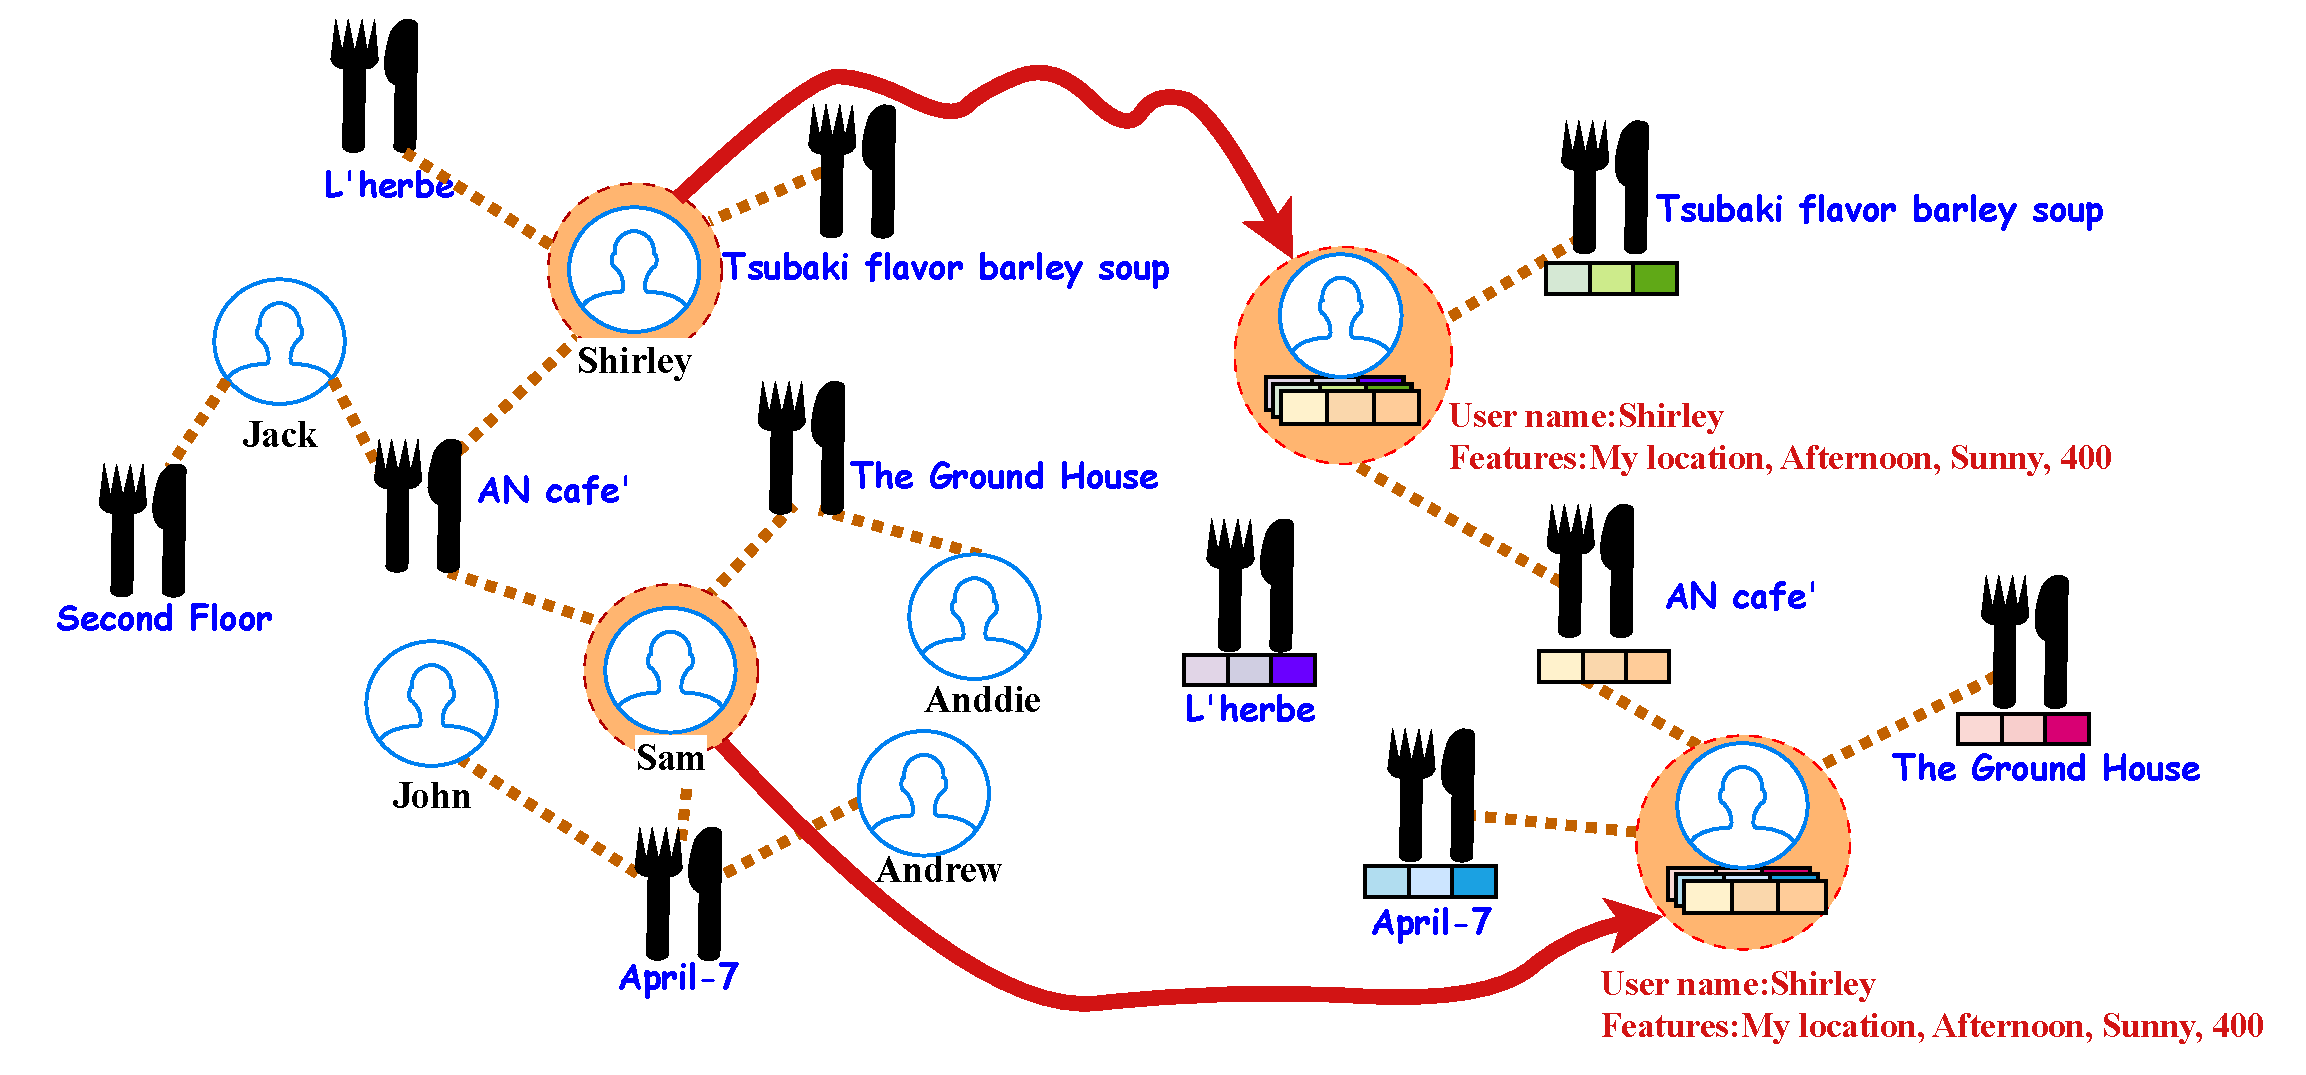
\includegraphics[width=0.5\textwidth]{img/bipartite_graph.pdf}
    \caption{推薦系統中的二分圖示意~\cite{bipratite_fig}}
    \label{fig-bipartite}
    \vspace{-0.35cm}
\end{figure}

如圖~\ref{fig-bipartite} 所示,節點可以分為兩類:使用者節點和餐廳節點,兩者節點類型的不同使得該圖同時為異質圖 (attributed heterogeneous graph)。本研究使用 Zhang 等人提出的 NIE-GCN 方法~\cite{NIE-GCN},從該資料集的二分異質圖中提取出更深層的連結信息,以預測顧客節點最感興趣的前 $k$ 個餐廳節點,進一步優化推薦精度。最終以歸一化折扣累積增益 (Normalized Discounted Cumulative Gain, NDCG) 和召回率 (Recall) 作為評估推薦系統表現的指標,為平台提供精確的推薦評估依據。
\begin{figure}[tbh]
    \centering
    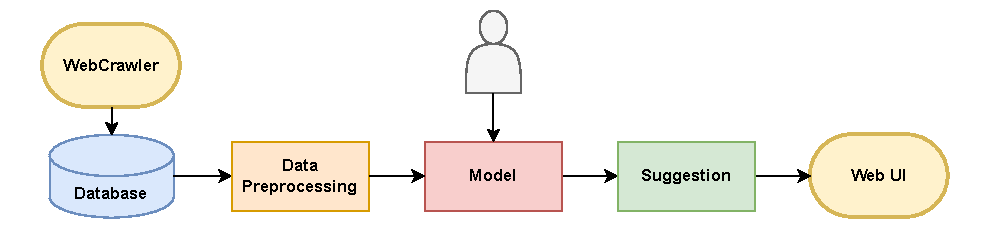
\includegraphics[width=0.5\textwidth]{img/flowg2.pdf}
    \caption{推薦系統架構圖}
    \label{fig-flowchart}
\end{figure}
本研究的架構如圖~\ref{fig-flowchart} 所示。首先,透過爬蟲技術從 Foodpanda 和 Google Maps 上獲取每個餐廳的資訊,並將這些資料儲存到資料庫中。接著進行基本的資料前處理,為模型的輸入做好準備。在使用者節點上,所包含的資訊如表~\ref{node-conetent} 所列。這些資訊經處理後會被輸入到模型中,最終生成推薦結果,並透過 Web UI 進行呈現。
\begin{table}[htbp]
    \centering
    \renewcommand{\arraystretch}{1.15}
    \setlength{\tabcolsep}{7.5pt}
    \begin{tabular}{|c|c|}
    \hline
    \textbf{節點類型} & \textbf{節點內容} \\ \hline
    使用者 & 當下位置、使用時間、天氣、預算 \\ \hline
    推薦餐廳 & 餐廳名稱、價位、評分、評論 \\ \hline
    \end{tabular}
    \caption{使用者與推薦餐廳的節點資訊}
    \label{node-conetent}
\end{table}
透過這些節點資訊,本研究可以針對不同使用情境生成個性化推薦,讓系統在多維度考量下更精確地滿足使用者需求。





    
\begin{figure*}[htbp]
    \centering
    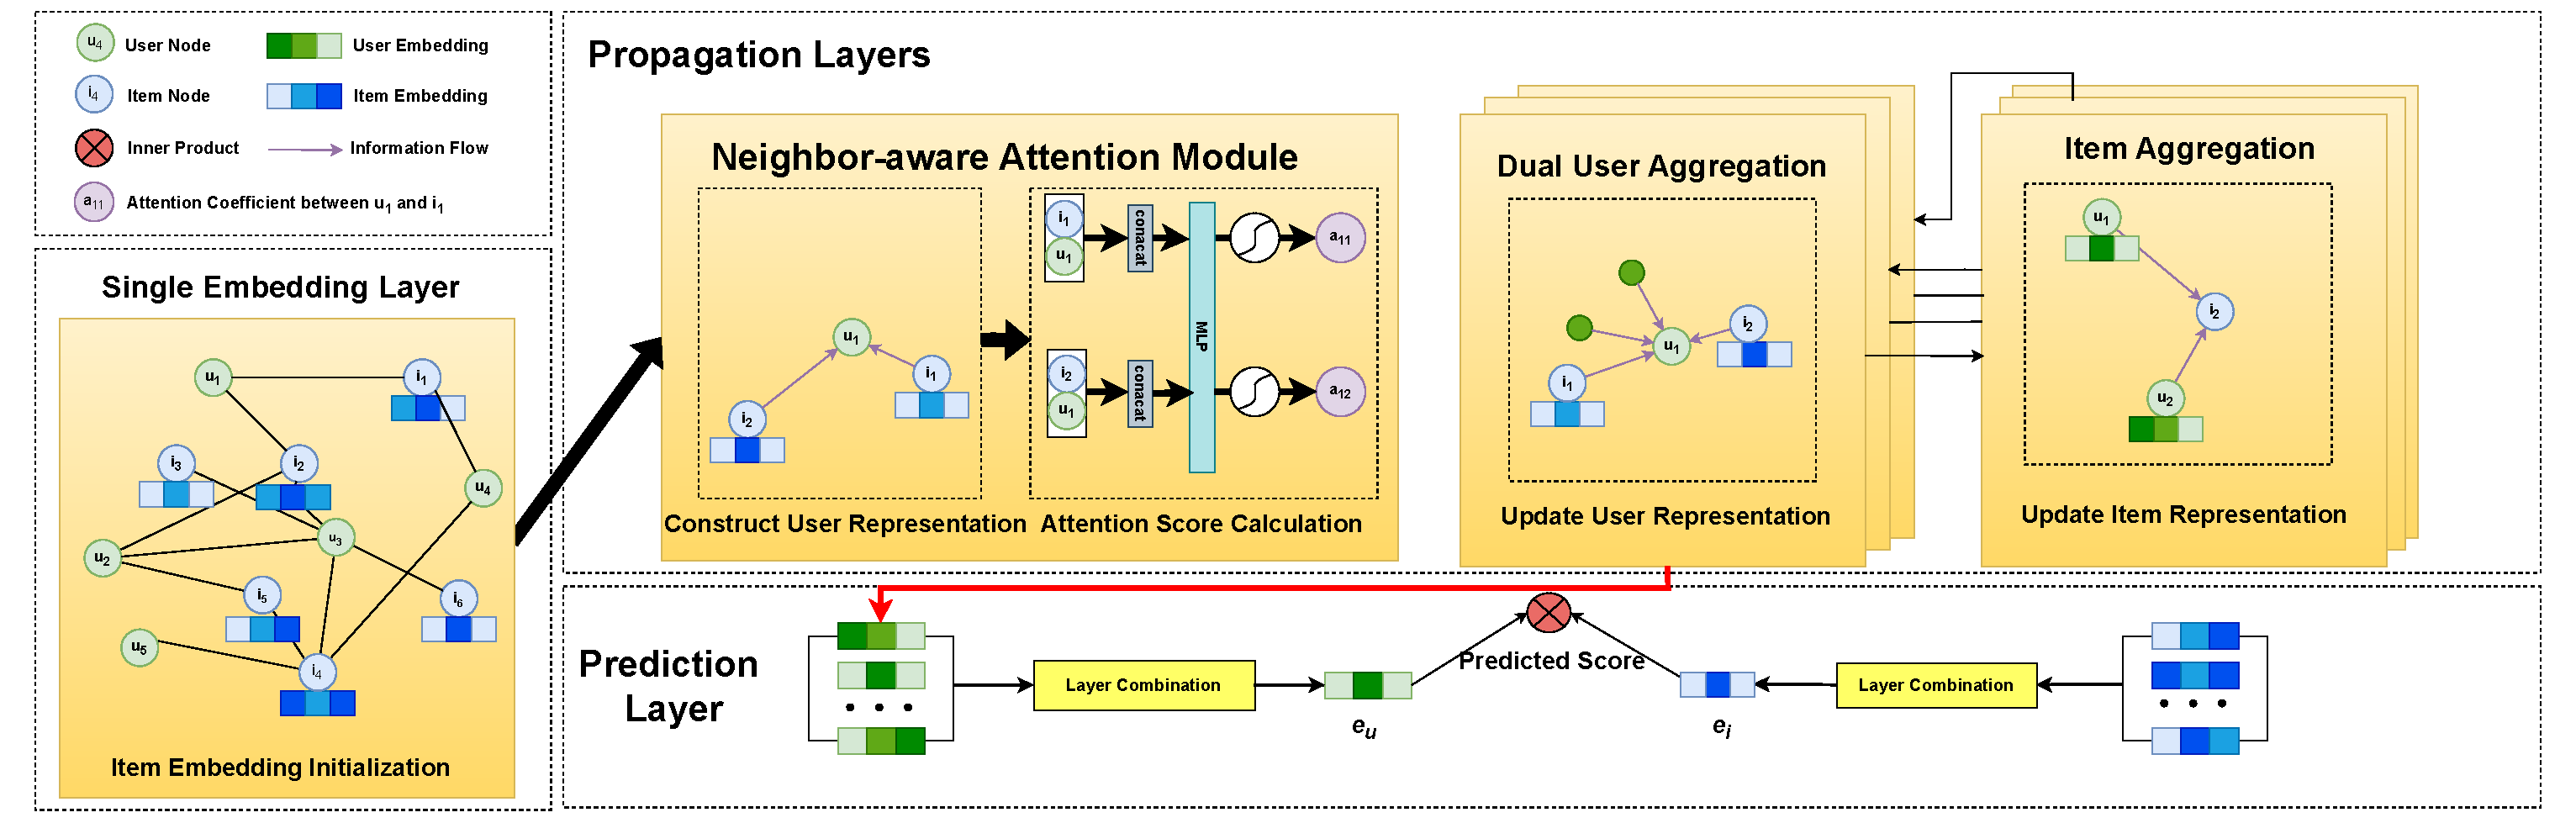
\includegraphics[width=\textwidth]{img/Model.pdf} % 替換成你的圖片檔案
    \caption{模型架構圖}
    \label{Model}
\end{figure*}

\section{Proposed}
\subsection{Single Embedding Layer}
    本研究所採用的~NIE-GCN\cite{NIE-GCN}~模型可拆解成幾個主要步驟如\xfig{Model},首先是對餐廳節點進行向量嵌入。第一步會針對每個餐廳節點 $i$ 生成一個嵌入向量 $e_i$,此向量位於 $d$ 維空間中,即 $e_i \in \mathbb{R}^d$。在嵌入過程中,所有餐廳節點的嵌入向量會被收集成一組矩陣 $E_I^{(0)}$,此矩陣表達了所有餐廳節點的初始嵌入狀態,如下式所示: 
    \begin{equation} 
        E_I^{(0)} = {e_{i_1}^{(0)}, e_{i_2}^{(0)},\cdots,e_{i_N}^{(0)}} \in \mathbb{R}^{N \times d}, 
    \end{equation}
    其中,$N$ 代表餐廳節點的總數,而 $d$ 則是嵌入向量的維度;上標 $0$ 表示第 0 層傳播的初始狀態。藉由得到每個餐廳節點的嵌入向量後,模型便可利用這些向量作為基礎,來進一步推斷每位使用者的偏好。因為每個使用者節點 $u$ 的鄰居必定為餐廳節點,故模型會透過與該使用者互動過的餐廳節點來推敲其個人喜好。

    在完成餐廳節點的嵌入後,第二步則是建構每位使用者節點的初始嵌入向量 $e_u^{(0)}$。此過程需要依賴與使用者節點 $u$ 相鄰的餐廳節點 $i$ 的嵌入向量 $e_i^{(0)}$。第 0 層的嵌入構造方式如下: 
    \begin{equation} 
        e_u^{(0)} = \sigma \left(\sum_{i \in N_u} \frac{1}{\sqrt{\vert N_u \vert \vert N_i \vert}}e_i^{(0)}\right), 
        \label{eq-e_u^0}
    \end{equation} 
    其中 $N_u$ 表示使用者節點 $u$ 的鄰居集合,而 $N_i$ 則代表餐廳節點 $i$ 的鄰居集合;$\sigma(\cdot)$ 是激活函數,選擇使用雙曲正切函數 (tanh)。透過這一層的加權平均,可以有效地融合使用者與其鄰近餐廳節點的特徵信息,以更準確地反映該使用者的行為特徵。

\subsection{Propagation Layers}
    完成初始嵌入後,下一步是計算每個使用者節點 $u$ 與其相鄰的餐廳節點 $i$ 之間的注意力分數 $\rho(u, i)$,藉此衡量不同鄰居節點的重要性。該分數計算方式如下: 
    \begin{equation} 
        \rho(u, i) = Q^T\sigma(W(e_u^{(0)}||(e_i^{(0)})+b)), 
    \end{equation} 
    其中 $W \in \mathbb{R}^{2d \times d}$、$Q \in \mathbb{R}^{1 \times d}$、$b \in \mathbb{R}^{1 \times d}$,這三個參數分別為注意力機制中的權重矩陣與偏置項。此處的 $\sigma(\cdot)$ 同樣為雙曲正切函數 (tanh),而 $||$ 則表示向量的串接操作。$\rho(u, i)$ 的分數越高,代表使用者 $u$ 與餐廳 $i$ 之間的關聯性越強。因此,透過該分數可以量化每個餐廳節點對於預測使用者偏好的貢獻度。

    為將注意力分數限制在 $[0,1]$ 的範圍內,利用 Softmax 函數對這些分數進行範圍歸一化處理,得到最終的注意力值 $\alpha(u, i)$。公式如下: \begin{equation} \alpha(u, i) = \frac{\exp(\rho(u, i))}{\left(\sum_{j \in N_u}\exp(\rho(u, j))\right)^{\beta}}, \end{equation} 其中 $\alpha(u, i)$ 代表了使用者節點 $u$ 與餐廳節點 $i$ 之間的最終注意力值。透過~$\alpha(u, i)$,每個使用者節點均能依據其鄰居的特徵,綜合考量注意力分數來完成向量更新。


    在初始嵌入狀態完成後,為進行更深層的特徵傳播,使用者節點 $u$ 的嵌入向量 $e_u^{(k)}$ 將在每一層根據其鄰居節點的資訊進行更新。使用者的嵌入向量 $e_u^{(k)}$ 的更新方式會依據先前計算出的注意力權重 $\alpha(u, i)$,並利用相鄰餐廳節點 $i$ 在上一層的嵌入向量 $e_i^{(k-1)}$ 進行加法聚合 (Add Aggregation)。此聚合方式可以有效融合鄰居的特徵信息,更新的計算公式如下: 
    \begin{equation} 
        e_u^{(k)} = \sigma\left(\sum_{i \in N_u} \alpha(u, i)e_i^{(k-1)}\right), 
    \end{equation} 
    其中,$\sigma(\cdot)$ 為雙曲正切函數 (tanh),$N_u$ 表示使用者節點 $u$ 的鄰居集合。透過加權聚合,使用者節點可以自適應地調整對不同鄰居特徵的重視程度,進一步增強模型對於不同使用者偏好的捕捉能力。

    同樣地,初始狀態後的餐廳節點的嵌入向量 $e_i^{(k)}$ 也會根據其相鄰使用者節點的嵌入進行更新。這個更新方式與\xeq{eq-e_u^0}~類似,餐廳節點 $i$ 的嵌入向量會根據其相鄰的使用者節點 $u$ 的嵌入向量 $e_u^{(k)}$ 進行加權平均,計算方式如下: 
    \begin{equation} e_i^{(k)} = \sigma \left(\sum_{u \in N_i} \frac{1}{\sqrt{\vert N_u \vert \vert N_i \vert}} e_u^{(k)}\right), 
        \label{eq-e_i} 
    \end{equation} 其中,$N_u$ 和 $N_i$ 分別表示使用者節點 $u$ 和餐廳節點 $i$ 的鄰居集合,並透過加權平均來控制每個鄰居對於嵌入向量的貢獻。此\xeq{eq-e_i}~與\xeq{eq-e_u^0}~中的加權項 $\frac{1}{\sqrt{\vert N_u \vert \vert N_i \vert}}$ 可以平衡不同鄰居數量對嵌入更新的影響,從而避免由於鄰居數量不均而引起的偏差。藉由此加權項,每個餐廳節點的嵌入向量都將根據與其相鄰使用者的特徵進行有效更新,從而更準確地反映餐廳與使用者間的潛在關係。

\subsection{Prediction Layers}
    在完成每一層使用者節點的嵌入向量 $e_u^{(k)}$ 和餐廳節點的嵌入向量 $e_i^{(k)}$ 的計算後,接下來的步驟是將這些嵌入向量進行聚合,以獲得最終的嵌入表達,在本研究將所有層的使用者嵌入向量和餐廳嵌入向量分別相加,計算公式如下: 
    \begin{equation} 
        e_u^* = \sum_{k=1}^{L} e_u^{(k)}, \quad e_i^* = \sum_{k=1}^{L} e_i^{(k)}, 
    \end{equation} 
    其中 $L$ 表示嵌入層的總數。這樣計算得到的 $e_u^*$ 和 $e_i^*$ 分別代表了使用者節點和餐廳節點的最終嵌入向量,這兩個向量綜合了多層的信息,能夠更全面地捕捉使用者與餐廳之間的潛在關聯。
    為了進一步評估使用者 $u$ 和餐廳 $i$ 之間的關聯性,將這兩個最終嵌入向量進行內積操作,為了將內積值限制在 0 到 1 的範圍內,引入了 S 型函數 (sigmoid function),計算公式如下: 
    \begin{equation} 
        \hat{y_{ui}} = f(u, i) = \sigma(e_u^{*T} e_i^*), 
    \end{equation} 
    其中,$\hat{y_{ui}}$ 表示模型對於使用者 $u$ 和餐廳 $i$ 之間關聯性的預測結果。S 型函數 $\sigma(\cdot)$ 將內積的結果映射到 $[0, 1]$ 的範圍,使得模型的輸出可以被解釋為一個機率值,表達使用者 $u$ 對餐廳 $i$ 的喜好程度。

\subsection{Model Optimization}
    本研究模型的目標函數採用貝氏個性化排序 (Bayesian Personalized Ranking, BPR),以實現使用者偏好排序的優化,具體公式如下:
    \begin{equation}
        \mathcal{L} = \sum_{(u, i) \in \mathcal{O^+}, (u, j) \in \mathcal{O^-}} -\ln\sigma(\hat{y_{ui}} - \hat{y_{uj}}) + \lambda\lVert \Theta \rVert_2^2,
    \end{equation}
    其中~$\mathcal{O^+}$ 和 $\mathcal{O^-}$~分別表示正樣本與負樣本的集合;正樣本為符合使用者偏好的項目,而負樣本為非偏好項目。$\sigma(\cdot)$ 是 S 型函數 (sigmoid function),可將輸出的範圍限制在 $[0, 1]$ 之間,用以衡量正樣本和負樣本之間的預測差距。此目標函數的設計旨在使正樣本的預測值 $\hat{y_{ui}}$ 高於負樣本的預測值 $\hat{y_{uj}}$,即期望 $\hat{y_{ui}}$ 越高越好,而 $\hat{y_{uj}}$ 越低越好,從而增強模型對正負樣本的區分能力。

    該目標函數包含了一項 L2 正則項,用於減少模型過擬合的風險。$\lambda$ 是 L2 正則化的係數,$\Theta = \{E_I, Q, W, b\}$ 表示模型中所有需要學習的參數集。通過引入正則項,模型的權重得以控制在合理範圍內,避免權重過大導致的模型複雜性增加。

    在計算過程中,預測差距 $\hat{y_{ui}} - \hat{y_{uj}}$ 的值範圍在 $[-1, 1]$,經過 S 型函數 $\sigma(\cdot)$ 映射後,範圍被壓縮到 $[0, 1]$。為了使目標函數在最大化的情況下實現梯度下降 (gradient descent) 訓練,對公式添加負號,這樣在取對數 $\ln$ 後,所有值為正,因此相當於最小化正的損失值,使得模型能夠通過梯度下降的方式進行有效優化。

\section{Experiment}
    \subsection{Data Preprocessing}
        \begin{figure}[tbh]
            \centering
            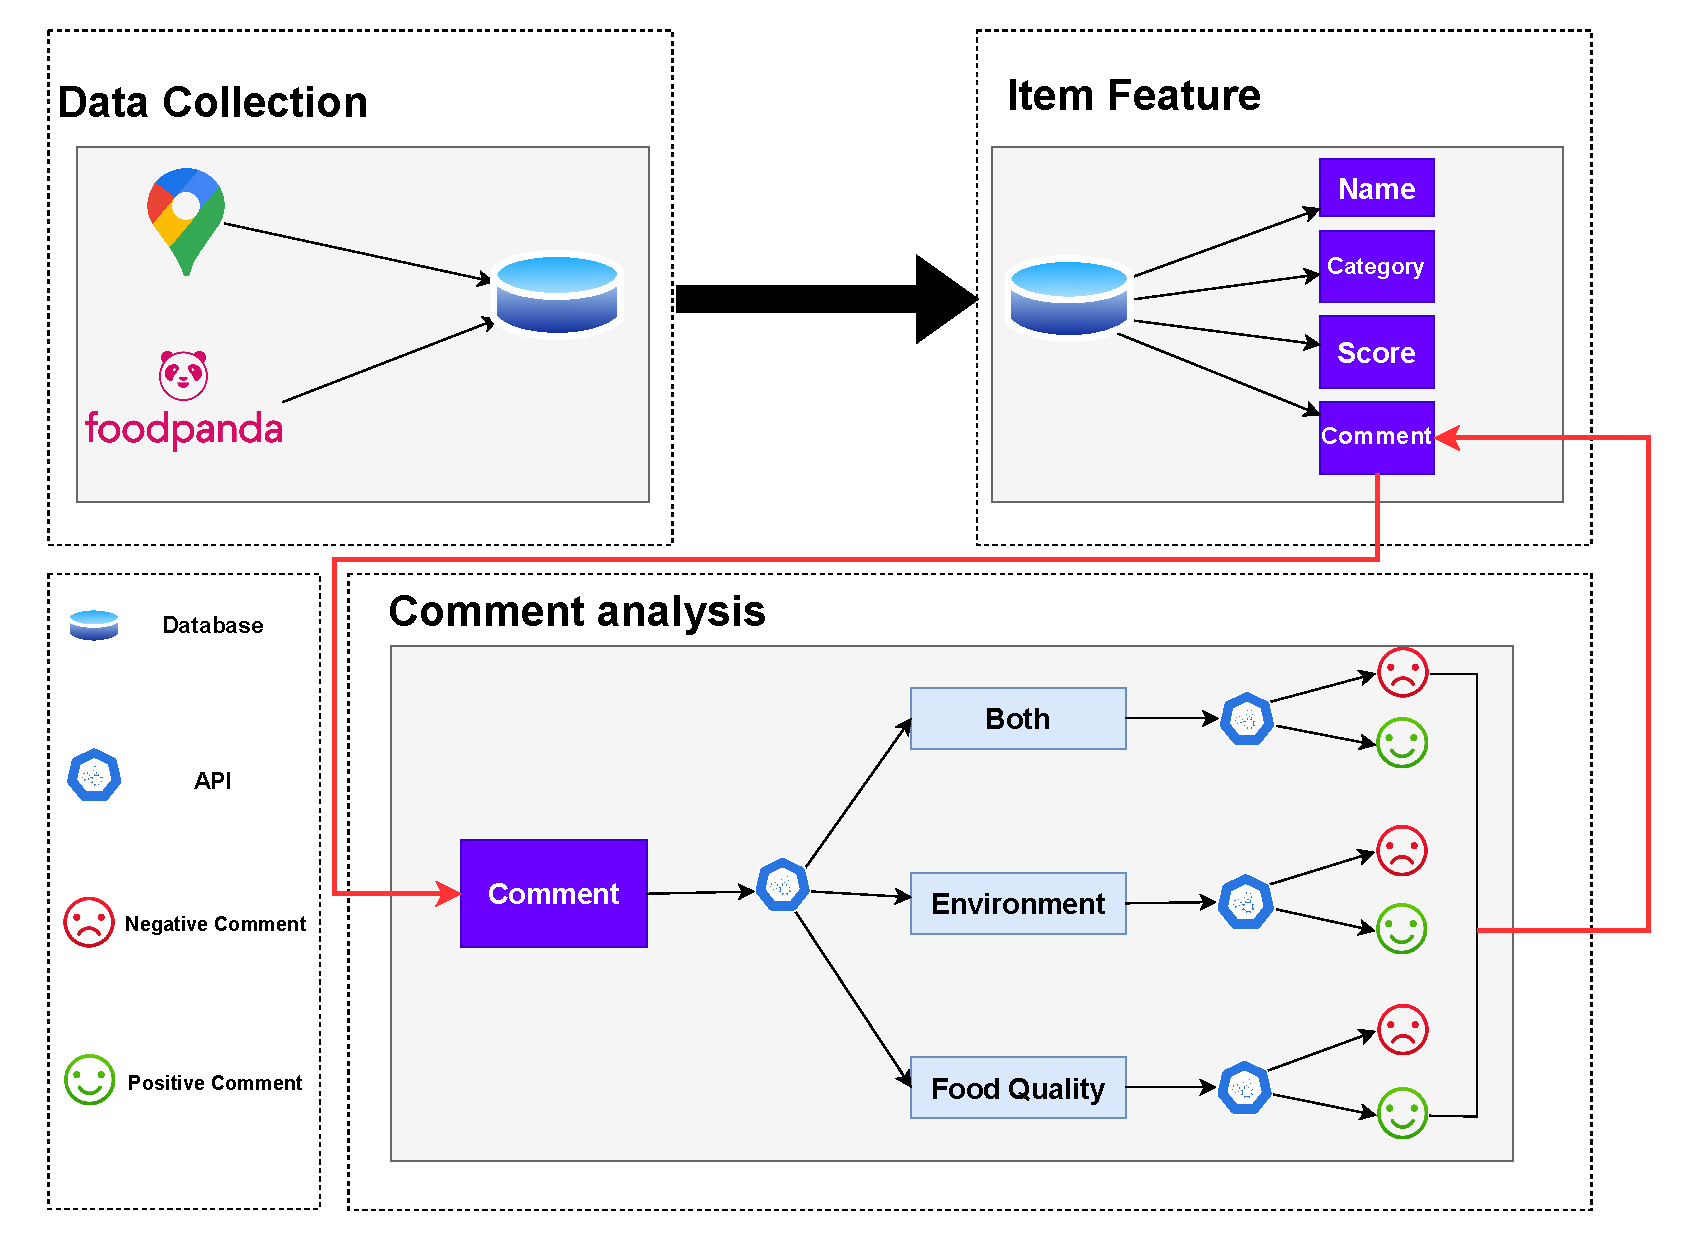
\includegraphics[width=0.5\textwidth]{img/preprocess.pdf}
            \caption{資料前處理架構圖}
            \label{fig-preprocess}
        \end{figure}
        本研究的資料前處理架構如 \xfig{fig-preprocess} 所示,利用爬蟲技術從 Foodpanda 和 Google Maps 獲取餐廳資料。每間餐廳的資料涵蓋了餐廳名稱、餐廳類型、評分以及顧客的評論。由於每家店通常會累積大量的評論,這些評論內容對於描述店家的品質、服務及顧客的體驗具有高度相關性。若將所有評論合併後再丟入 GPT-4 進行分析,可能會因評論主題多樣性導致訊息混雜,進而影響模型的微調(Fine Tuning)效果。當不同主題的評論一起進行訓練時,模型可能難以識別每個特徵的意圖,進而影響結果的精準度。

        為提升模型的針對性,本研究首先將評論依主題分為三類:餐點品質、店內環境氣氛,以及兩者皆有的綜合評價。針對這三類評論,我們分別對每一類進行獨立的 LLM 微調。這種獨立的微調方法有助於每個模型專注於該主題的特徵,避免不同主題之間的訊息干擾。對於餐點品質類評論,模型學習專注於食物的口感、質量及呈現;對於店內環境氣氛的評論,模型則聚焦在用餐氛圍、環境設計及舒適度等描述上;而綜合評價類別則幫助模型掌握顧客的整體體驗。通過分開微調,每個模型能精確捕捉該主題的特徵表現,使得每一類評論的處理結果更具針對性。\color{blue}

        完成初步主題分類與獨立微調後,針對每一類主題中的評論再進行情感分析,以判斷其情感取向為正面或負面。由於共有三種初步主題分類 \( C = \{ c_1, c_2, c_3 \} \),且每個分類中進一步區分為正面(\( P \))與負面(\( N \)),因此共有六種情感分類,定義為集合:
        \begin{equation}
            S = \{ c_1^P, c_1^N, c_2^P, c_2^N, c_3^P, c_3^N \},
            \label{eq-classification}
        \end{equation}
        其中 \( c_1 \) 表示"餐點品質"、\( c_2 \) 表示"店內環境氣氛"、\( c_3 \) 表示"綜合評價";\( P \) 表示該主題分類下的正面情感,\( N \) 表示該主題分類下的負面情感。
        \[
        \mathbf{e}(s) \in \mathbb{R}^d,
        \]
        其中 \( d \) 為嵌入向量的維度。
        
        假設某店家 \( j \) 有 \( n_j \) 條評論,每條評論 \( i \) 的初步主題分類為 \( c_{j,i} \in C \),且每個主題分類對應的權重為 \( w(c_{j,i}) \)。對於第 \( i \) 條評論,其嵌入向量為 \( \mathbf{e}_{j,i} = \mathbf{e}(c_{j,i}) \),權重 \( w(c_{j,i}) \) 根據三種分類具體設定,滿足:
        \begin{equation} 
            w(c) = 
            \begin{cases} 
                w_{1}, & \text{若 } c = c_1, \\ 
                w_{2}, & \text{若 } c = c_2, \\
                w_{3}, & \text{若 } c = c_3, 
            \end{cases} 
            \label{eq-weight} 
        \end{equation}
        其中 \( w_1, w_2, w_3 \) 分別表示三種主題分類的重要性權重。
        本研究對所有評論的嵌入向量進行加權平均:
        \begin{equation} 
            \mathbf{e_j} = \frac{\sum_{i=1}^{n_j} w(c_{j,i}) \cdot \mathbf{e}_{j,i}}{n_j},
            \label{eq-embedding} 
        \end{equation}
        其中 \( \mathbf{e_j} \) 表示店家 \( j \) 涵蓋所有評論所得出之最終的評論嵌入向量。
    \subsection{Dataset}

        
\color{black}
\section{Conclusion}
我們提出了一種新穎的方法,利用NIE-GCN模型來解決餐廳推薦系統的挑戰。該模型能有效從二分異質圖中提取更深層的關聯信息,並精確預測顧客節點最感興趣的前 $k$ 個餐廳節點。我們的方法在推薦系統中表現出色,Recall@5 達到 0.810,NDCG@5 則達到 0.917,顯示出該模型在推薦任務中的優越性能。

本研究的主要挑戰在於資料集的建立。由於無法透過爬蟲從 Foodpanda 和 Google Maps 等平台獲取用戶與餐廳的互動資料,我們採用了問卷調查的方式收集資料。但此方法導致資料量不足,且無法完全保證資料的真實性。問卷調查無法直接獲得用戶與餐廳的互動資料,因此我們只能藉由用戶填寫的興趣類別來模擬實際的互動關係。此外,如何將每個店家的評論與評分轉換為適合分析的特徵向量,也是我們面臨的一大挑戰。研究結果顯示,NIE-GCN模型在提升餐廳推薦系統性能方面具有巨大潛力。未來的研究應著重於建立更大規模且更具真實性的資料集,例如與業界合作,進一步驗證並優化所提出的方法。
\color{black}
{
    \small
    \bibliographystyle{IEEEtran}
    \bibliography{main}
}

\end{CJK}  % 在 document 结束时关闭中文支持
\end{document}
